\section{Case Study: ThingSat}
\label{sec:case-study}

%\subsection{Overview}
% \paragraph*{Mission Goal:} in-orbit observation of glaciers in Europe and in Polynesia.
% \paragraph*{Approach}: rent "rack" space as payload on a CubeSat (SatRevolution).

The Thingsat project~\cite{git:thingsat-repo} aims to benchmark the LoRa links in the context of
space-ground communication for several frequency bands and demonstrate the
effectiveness of that technology inside a LEO (Low Earth Orbit) cubesat.

Thingsat is deployed as a payload hosted on a shared 3U CubeSat: \href{https://space.skyrocket.de/doc_sdat/stork-1.htm}{STORK-1} from the polish start-up \href{https://www.satrevolution.com/}{SatRevolution}. The cubesat was launched on January 13th, 2022,currently in orbit at an altitude of 525 km (see its 
\href{https://www.n2yo.com/database/?q=STORK-1\#results}{Two-Line Elements}).

The Thingsat payload now in orbit is used for Ocean level monitoring.
\todoEB{reformulate/check this bit.}
However, its design can be adequate for a wider variety of use cases, in Earth science academic research (e.g. melting of glaciers, pirate fishing...) and in the industry for companies using geographically dispersed devices (e.g. monitoring of tank ships...). 

\iffalse
Thus we designed a space electronic board with two LoRa transceivers and a patch
antenna operating in 868MHz and 2.4GHz. 
This payload is hosted in a shared 3U
CubeSat - \href{https://space.skyrocket.de/doc_sdat/stork-1.htm}{STORK-1} from
the polish start-up \href{https://www.satrevolution.com/}{SatRevolution}. The
cubesat was launched on January 13th, 2022 on a near-polar orbit at an
altitude of 525 km (See
\href{https://www.n2yo.com/database/?q=STORK-1\#results}{Two-Line Elements}).
\fi


\begin{figure}[t]
    \centering
    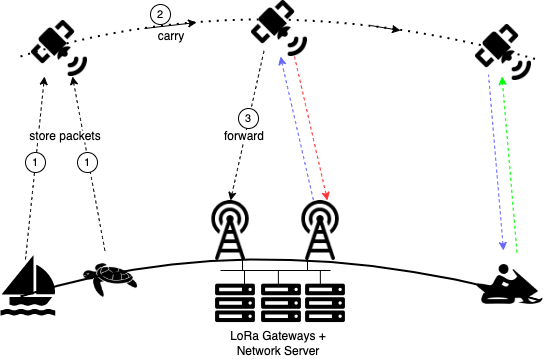
\includegraphics[width=0.5\textwidth]{Figures/thingsat-dtn.png}
    \caption{ThingSat in-orbit communication patterns.}
    \label{fig:thingsat-comm}
\end{figure}


% \paragraph*{High-level overview of Segments}

\subsection{Distributed System Architecture}

The figure \ref{fig:thingsat-archi} describes the Thingsat deployment components, which gives an
overview of a typical cubesat ecosystem hosting a payload, whereby the interaction with this payload traverses untrusted elements.

\subsection*{Low-power Space Segment} 
% \paragraph*{Space Segment Description}
The Space Segment comprises of the on-board computer (OBC) and hosted payloads, interconnected via a CAN bus, which share resources on the cubesat.
\begin{itemize}
\item The OBC provided by the satellite operator consists of 
a microcontroller with all its subsystems to operate the cubesat :
the Attitude Determination and Control System (ADCS),
the communication subsystems (UHF/VHF/S-band for uplink/downlink and antennas),
the power subsystem (Battery Management, Energy Harvesting with Solar Panels, Auxiliary Power Supply). 

\item We designed the Thingsat payload, using a low-power ARM Cortex-M microcontroller (STM32) and open source firmware based on RIOT~\cite{baccelli2018riot}. The Thingsat payload embeds both a
\href{https://www.semtech.com/products/wireless-rf/lora-gateways/sx1302}{Semtech SX1302 transceiver} for communications on the 863-870 MHz band and a
\href{https://www.semtech.com/products/wireless-rf/24-ghz-transceivers/sx1280}{Semtech SX1280 transceiver} for communications on the 2400-2500 MHz band. Furthermore we designed a corresponding dual-band patch antenna (868MHz, 2.4GHz).
To give an idea, when active and using the 863-870 MHz band, the
Thingsat payload consumes at 3.3V : 
(i) 90 mA in standby, 
(ii) 110 mA during a frame reception (RX) and 
(iii) 300 mA during a frame transmission (TX) at 27 dBm.
\end{itemize}

% \paragraph*{Ground Segment Description}
% \paragraph*{Control Segment} % Francisco: not sure if its the right name

\subsection*{Ground Segment}
For the Ground Segment, elements which communicate with the Thingsat payload are of multiple nature. are of the cubesat operator relies on 
\begin{itemize}
\item The cubesat operator provides a number of Ground Stations\footnote{not necessarily owned by the cubesat operator} to communicate via UHF/VHF with the OBC, and indirectly with the payload. 
A Command \& Control Center is also provided to operate the cubesat (telecommand/telemetry) which acts as broker for payload maintainers to interact with the hosted payload.
\item Additionally, we designed and deployed and maintain LoRa-based  \href{https://github.com/thingsat/tinygs_2g4station}{Thingsat ground stations}, which can communicate with the Thingsat payload directly via LoRa. These stations are based on a low-cost ESP32 microcontroller, and an SX1280 transceiver for LoRa communication at 2.4GHz, also running an open source firmware based on RIOT.
\end{itemize}
% \paragraph*{OBC \& Payload Communication Bus}

% \paragraph*{Payload Description}: tenant status, energy budget, on time etc.
% - OBC -> SatRev controlled
% - Payload -> Full Control

\subsection{Communication Characteristics Overview}
\label{sec:thingsat-comm-characteristics}
% \paragraph*{link-budget Mission Control}: delivering and communicating mission
% files, delivering software updates, latency, etc.

The Thingsat payload communicates either directly via low-power WAN, or indirectly via the UHF/VHF link provided by the cubesat's OBC.

\paragraph*{Direct communication patterns via low-power WAN}
Thingsat can communicate directly with LoRa. %, with LoRa network elements on the ground.
In principle, although it is not used as such so far, this communication link could also be used to transport some software updates.
Low-power WAN communication patterns are illustrated in \autoref{fig:thingsat-comm}.
The Thingsat payload may act in turns as either 
(i) a Sat-IoT end-device (ED) that will send LoRa frames to terrestrial LoRaWAN gateways or Thingsat ground stations (GS), or 
(ii) an in-orbit LoRa sniffer, or 
(iii) a store-carry-and-forward LoRa gateway.

Patterns (i) and (ii) allow to benchmark simple ground-space LoRa links by
computing statistics over multiple sent/received frames. 
Pattern (iii) is a more
complex scenario: the satellite stores packets received from GS/ED and deliver
them once GS/ED destinations are inside the footprint of the satellite.

\paragraph*{Indirect communication characteristics via UHF/VHF}
Communication with cubesats are typically done on amateur frequency
bands (UHF/VHF) with typically low data rates ranging from 9.6kbps to
100kbps. 
Generally, over a given ground station, a polar LEO satellites passes 2 to 4 times per day. The duration of the communication window for each pass is approximately of 5 to 10 minutes. 

In the particular case of Thingsat, the cubesat operator provides only 2 ground stations (both located in Europe) to interact with the cubesat, which communicate via a 10-kbps UHF/VHF link.
The throughput that can be exchanged during a day is thus roughly 1500KB (corresponding to 2 GS x 2
passes/day x 5-min pass duration x 10kbps).
 However, note that this throughput must be shared between communications to/from the OBC
(for telecommand/telemetry/update) and to/from hosted payloads. 
In practice, to give an
idea, the total communication budget available for Thingsat via UHF/VHF is thus 300KB per day. \todoOA{See with SR for details}


% \paragraph*{link-budget Mission}: communication between OBC and Payload, payload
% active time for communication with ground segments.
\iffalse
Regarding the communication with the OBC, an API is provided to the hosted
payload to read/write data with the data handling module of the cubesat as well
as interacting with its subsystems. Indeed, to carry out a provisioned mission,
the payload needs information from the OBC : awaiting uploaded
instructions/files, GPS, time, ADCS, time before shutdown, ...
\fi

\paragraph*{Intermittent communication/power supply}
Last but not least, the Thingsat payload is not powered ON all the time.
On such a cubesat, the power available is only enough for one active payload at a time. 
%The mission of the STORK constellation is earth observation. So each STORK cubesat is equipped with an imager~\cite{wiki:SatRevolution} which has its own missions.
The OBC is in charge of turning on the relevant payload according to a schedule uploaded from the ground station. 
Typically, for a 3U, 1U is dedicated to the OBC and the remaining 2U, available for host payloads, is divided in 8 slots.
The Thingsat payload occupies one slot out of 8 and would be turned ON 12.5\% of the time. 
It is obviously an average since the schedule to turn on payloads relies on multiple factors (mission specificities, regulations, battery level). 
% \todoEB{reformulate/check this bit: what average percentage of the time is the payload powered?}
This intermittent power supply, combined with orbiting and radio range limitations impacts the intermittence of network connectivity to/from the Thingsat payload.

% solar panel rechargé la moitié du temps
% 1U pour l'OBC + 2U pour le reste avec 8 slots dont Thingsat a 12.5% du temps de l'énergie
% les images c est pas tout le temps (pas quand on survole les russes) allumé aussi de la région of interest
% donc il faut aussi respecter la régulation des émissions et collecte des données

\subsection{Hosted Payload Software Updates Requirements}
\label{sec:thingsat-update-req}

% \paragraph*{Why?}: timeline for deployment, CoVID context, etc. making it impossible
% to deliver a fully functional device in time. Need to update the firmware remotely
% and in orbit.

The data exchanged by the Payload Maintainer with the Thingsat payload consists in 
\begin{enumerate}
    \item Firmware updates (Uplink): fix bugs, add/improve functionality, $\sim 200kB$ per FW, 1 FW/month,
    \item Mission description (Uplink): to update configuration scenarios/scripts, $\sim 700B$ per mission, 10 missions/day,
    \item Mission results (Downlink): radio metadata, frame stats, collected LoRa frames, $\sim 700B$ per mission, 
    \item Diagnosis (Downlink): debug failed missions/updates, $\sim200B$ per mission.
\end{enumerate} 

% 1 mission = envoi de frames sur une zone (fichier jetable pour l'instant, )
% combien de groupes de missions envoyés par semaine ? --> quelle taille va être sécurisée par SUIT ?
% 10 missions par jour vérifiée par SUIT

% sequence mission description : .EXP Experiment_t                     1820     2KB                                          
% .RES Result_t                         717                                                
% .PKT (32kB) et .TMP (local pour forward)  PktFile_t                    2858     x  256 = 730 KB
% chaque mission = .RES + .PKT only metadata + truncated pkts if too long (?)   
% .DIA Diag_t                           222

% https://gricad-gitlab.univ-grenoble-alpes.fr/thingsat/thingsat-modules/-/blob/master/modules/mission/include/lgw_pkt_rx.h#L59
% https://gricad-gitlab.univ-grenoble-alpes.fr/thingsat/thingsat-modules/-/blob/mission_scenario/modules/mission/include/pktfile.h#L65


% The ability to reprogram the cubesat in orbit is essential for academic projects like Thingsat. First the design, development and deployment life-cycles of cubesat projects are quite short and the financial budget in academic projects is limited. Secondly the academic development team (students, professors, engineers) are at best experts in their respective domain but not necessarily familiar with space systems. Those constraints makes it impossible to deliver a fully functional device in time. The COVID context aggravated the situation with forced remote working, electronic component shortages and delayed shippings. 

% \paragraph*{What needs updates}: Missions ? 

% Software update consists in above parts (1) and (3). To give an idea
% for (1) the size of mission files is in the order of 10kBytes and the frequency of updates is roughly once a month. 
% To give an idea 
% for (3) the size of firmware updates is in the order of 200kBytes and the frequency of updates is roughly XXX( WITHOUT SUIT!!!).

% \todoOA{Check numbers above. Be more specific on those files (discuss with Didier + give typical size of files, frequency of updates (and show sample config file?)}

%sIn-orbit software updates must allow for updating radio drivers, the evolution of missions scenarios or configurations file format, bug resolutions ...
% Fortunately the use of RIOT-OS greatly facilitates the process to update softwares \textcolor{red}{but still needed adaption to our context}.

% \paragraph*{Communication Chain}: how are new firmware, payloads delivered,
% who has access, etc..
\iffalse
At last, the update of softwares like the Firmware (FW) for instance goes
through the following steps : i) the FW is uploaded to the cubesat by the
payload maintainer (PO) through one of the cubesat operator (CO) ground
stations, ii) once the payload is turned on and reset, it asks the OBC for any
awaiting files/instructions to execute, iii) the OBC uploads the FW chunk by
chunk to the payload and iv) the FW update is triggered by the payload. This
process provided by the CO going through the untrusted parts identified in
figure \ref{fig:thingsat-archi} led us to provide the secured process detailed in the
next section.
\fi

\begin{figure}[t]
    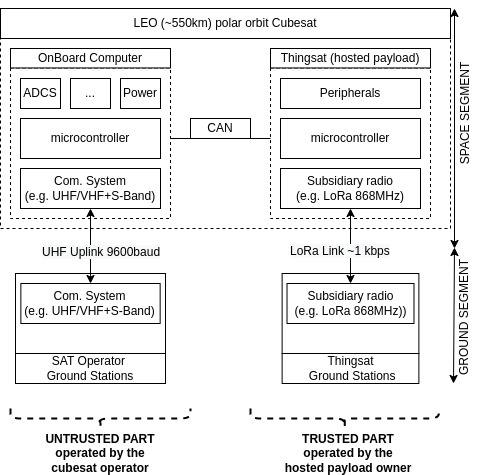
\includegraphics[width=0.5\textwidth]{Figures/globecom-thingsat-mods.jpg}
    \caption{ThingSat hosted payload: deployed components and architecture.}
    \label{fig:thingsat-archi}
\end{figure}